% CSE 561 project report: shortest-path bypass for small flows in Spraypoint.
% Build from this folder with `latexmk`; the PDF lands next to this file.  Figures and the tables
% in tables/, once included, are generated by experiments/analysis/report_figures.py.
\documentclass[11pt]{article}

\usepackage[T1]{fontenc}
\usepackage[utf8]{inputenc}
\usepackage{lmodern}
\usepackage[margin=1in]{geometry}
\usepackage{microtype}
\usepackage{amsmath,amssymb,mathtools}
\usepackage{booktabs,tabularx,array}
\usepackage{graphicx}
\usepackage{caption,subcaption}
\usepackage{enumitem}
\usepackage{xcolor}
\usepackage{tikz}
\usetikzlibrary{arrows.meta,positioning,calc}
\usepackage[numbers,sort&compress]{natbib}
\usepackage[hidelinks]{hyperref}

\setlist{itemsep=0.2em,topsep=0.3em}
\setlength{\parskip}{0.4em}
\captionsetup{font=small,labelfont=bf}
\newcolumntype{L}{>{\raggedright\arraybackslash}X}
\graphicspath{{figures/}}
% File and program names, which may break at / and - to fit the line.
\newcommand{\file}[1]{\path{#1}}
\newcommand{\sumu}{\textstyle\sum_i \mu_i}
% Section references read as "Section 3" or "Appendix A".
\newcommand{\secref}[1]{Section~\ref{#1}}
\newcommand{\appref}[1]{Appendix~\ref{#1}}

\title{Shortest-Path Bypass for Small Flows in Spraypoint}
% One block, so the course line is centered under all three names, not the last one.
\author{Duc Thanh Vinh Nguyen \qquad Yusong Yan \qquad Cheng Peng\\[0.6em]
  \normalsize CSE 561: Computer Communication and Networks\\
  \normalsize University of Washington, Autumn 2026}
\date{November 2026}

\begin{document}
\maketitle

\begin{abstract}
RNG builds a datacenter network as a flat random graph of top-of-rack routers, and its routing protocol, Spraypoint, sends every packet through a random neighbor first. That spreads load well, but it sends even a tiny message between two directly connected racks over two to five hops. We test a \emph{bypass} that routes small flows on the shortest path instead. Using an ns-3 simulation of a 256-router fabric, flow-level computations on the paper's 1{,}000-router fabric, and analytical models extended from the RNG paper, we measure how much the bypass speeds up small flows, what it costs the rest of the traffic under uniform and worst-case traffic, and when that cost outweighs the gain.

\end{abstract}

\section{Introduction}
\label{sec:intro}

RNG~\cite{rng} builds a datacenter fabric as a single layer of top-of-rack routers wired as a random graph. Its routing protocol, Spraypoint, sprays each flow to a random neighbor before pointing it at the destination, which spreads every pair's traffic over dozens of paths. That suits throughput, but much datacenter traffic is small and latency-sensitive (RPCs, key-value lookups, control messages), and for it what matters is the tail of the flow completion time (FCT). Spraying sends even a message between two directly connected racks over three or four hops, and each hop is another queue to wait in and another place to be dropped.

We test a \emph{bypass} that lets small flows skip the spray and take a shortest path, which the paper warns concentrates traffic on direct links:

\begin{quote}
\emph{On an RNG fabric, does routing small flows on shortest paths reduce their tail latency? What does it cost the rest of the traffic, and when does the cost outweigh the gain?}
\end{quote}

We answer with an ns-3 simulation, flow-level computations at the paper's scale, and the paper's analytical models extended to the bypass (\secref{sec:models}), testing four hypotheses:
\begin{description}[leftmargin=2.5em,style=nextline]
  \item[H1 (latency)] The bypass cuts small flows' FCT tail, most between neighbors, which cross one queue instead of two to five (\secref{sec:h1}).
  \item[H2 (no free lunch)] Other traffic barely notices at low small-flow volume, but as the small flows' share of bytes or the load grows, direct links become hotspots and past a crossover the bypass makes things worse (\secref{sec:h2-uniform}, \secref{sec:h2-perm}).
  \item[H3 (reach)] Only about $d/(n-1)$ of router pairs are neighbors, so reaching most small flows means covering every pair, which raises the hotspot risk (\secref{sec:h3}).
  \item[H4 (overhead)] A switch pays one extra table lookup, negligible next to queueing; we argue this but do not measure it (\secref{sec:bypass}).
\end{description}

\section{Background}
\label{sec:background}

RNG connects $n$ routers directly, with no spine layer, each with $d$ fabric links wired so the graph behaves like a uniformly random $d$-regular graph; at the paper's defaults, which our models use, $n = 1000$ and $d = 64$. Shortest paths on such a graph use only a handful of the $d$ links between two routers, so Spraypoint spreads each pair's traffic in two phases (\autoref{fig:rings}):
\begin{enumerate}
  \item \textbf{Spray.} The source router $s$ hashes the flow to one of its $d$ neighbors, ignoring the destination.
  \item \textbf{Point.} Around each destination $t$, routers form rings: WP0 holds $t$'s $d$ neighbors, WP1 the $p = 4$ waypoints each WP0 router picks among its neighbors, the inner ring (IR) every other router touching WP1, and the outer ring (OR) the rest, almost none. Each router splits traffic over $h = 2$ next hops in the next ring inward, so traffic walks inward one ring per hop.
\end{enumerate}

\begin{figure}[ht]
\centering
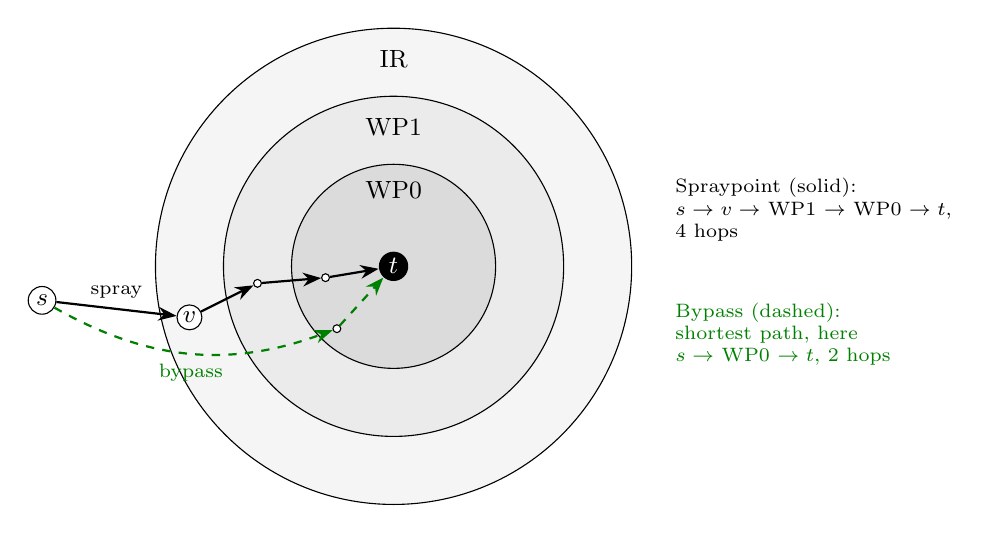
\begin{tikzpicture}[scale=0.72, every node/.style={font=\small}]
  \draw[fill=black!4] (0,0) circle (4.2);
  \draw[fill=black!8] (0,0) circle (3.0);
  \draw[fill=black!14] (0,0) circle (1.8);
  \node[circle, fill=black, text=white, inner sep=1.5pt] (t) at (0,0) {$t$};
  \node at (0, 1.35) {WP0};
  \node at (0, 2.45) {WP1};
  \node at (0, 3.65) {IR};
  \node[circle, draw, fill=white, inner sep=1.5pt] (s) at (-6.2, -0.6) {$s$};
  \node[circle, draw, fill=white, inner sep=1pt] (v) at (-3.6, -0.9) {$v$};
  \node[circle, draw, fill=white, inner sep=1pt] (w1) at (-2.4, -0.3) {};
  \node[circle, draw, fill=white, inner sep=1pt] (w0) at (-1.2, -0.2) {};
  \draw[-{Stealth}, thick] (s) -- node[above, font=\scriptsize] {spray} (v);
  \draw[-{Stealth}, thick] (v) -- (w1);
  \draw[-{Stealth}, thick] (w1) -- (w0);
  \draw[-{Stealth}, thick] (w0) -- (t);
  \node[circle, draw, fill=white, inner sep=1pt] (n) at (-1.0, -1.1) {};
  \draw[-{Stealth}, thick, dashed, color=green!50!black] (s) to[bend right=25] node[below, font=\scriptsize] {bypass} (n);
  \draw[-{Stealth}, thick, dashed, color=green!50!black] (n) -- (t);
  \node[align=left, font=\scriptsize, anchor=west] at (4.8, 1.0) {Spraypoint (solid):\\$s \to v \to$ WP1 $\to$ WP0 $\to t$,\\4 hops};
  \node[align=left, font=\scriptsize, color=green!50!black, anchor=west] at (4.8, -1.2) {Bypass (dashed):\\shortest path, here\\$s \to$ WP0 $\to t$, 2 hops};
\end{tikzpicture}
\caption{Spraypoint's rings around a destination $t$. The spray lands on a random neighbor $v$ of the source $s$, usually in the large inner ring, and the flow then walks inward one ring per hop. The bypass (dashed) takes a shortest path instead.}
\label{fig:rings}
\end{figure}

\paragraph{The paper's models.} On a random graph a router's neighbor is close to a uniformly random router, so the spray lands in a ring with probability that ring's size over $n$. We use three of the paper's results (§7 and Appendices E--G of~\cite{rng}).
\begin{itemize}
  \item \textbf{Path length} (Model 7.2). Most paths take 4 hops, because most routers are in IR:
\begin{center}
\small
\begin{tabular}{@{}lccccc|c@{}}
\toprule
Spray lands in & $t$ & WP0 & WP1 & IR & OR & \\
Hops & 1 & 2 & 3 & 4 & 5 & Mean \\
Probability & 0.1\% & 6.4\% & 25.6\% & 67.9\% & $\approx 0$ & \textbf{3.61} \\
\bottomrule
\end{tabular}
\end{center}
  \item \textbf{Path diversity} (Model 7.1). In exchange, each pair gets about $d(1 - e^{-h}) \approx 55$ of a possible 64 edge-disjoint paths, and traffic reaches $t$ through many of its neighbors (high \emph{fan-in}).
  \item \textbf{Throughput} (Model 7.3). The paper measures throughput by \emph{oversubscription} $r$: every router can send $1/r$ of its full rate at once without overloading any link. The worst case is a \emph{permutation}, where every router sends to one partner~\cite{namyar}, and the paper's LP, which splits each pair's traffic over its paths in the best way, gives $r = 3.25$. Model 7.3 approximates the LP by filling the shortest paths first. With $\mu_i d$ the rate, in links' worth, that $s$ can send to $t$ on $i$-hop paths, $r = 1/\sumu$:
\begin{center}
\small
\begin{tabular}{@{}lccccc@{}}
\toprule
& $\mu_2$ & $\mu_3$ & $\mu_4$ & $\mu_5$ & Sum \\
\midrule
Value & 0.064 & 0.131 & 0.111 & $\approx 0$ & \textbf{0.306} \\
Links' worth & 4.1 & 8.4 & 7.1 & 0 & \textbf{19.6} \\
\bottomrule
\end{tabular}
\end{center}
  so $r \approx 3.27$.\footnote{The paper's printed $\mu_5$ formula uses the share of routers in IR where the share in OR is meant; we read it as a typo, and our implementation uses OR.} The $\mu_2$ paths, $s \to \text{WP0} \to t$, about $d^2/n = 4.1$ per pair, are also the pair's shortest paths.
\end{itemize}

The best split is a bound: switches split traffic \emph{evenly} over their next hops (ECMP), so we model the bypass under both (\secref{sec:models}).

\section{The small-flow bypass}
\label{sec:bypass}

A \emph{small flow} is one whose size is at most a threshold, 10\,KB in most of our experiments. The sending host marks every packet of a small flow, and its ACKs, with a DSCP code point (AF11), so routers can tell small-flow packets apart without inspecting anything else. Every router forwards a marked packet to a neighbor one hop closer to the destination, hashing the flow over all such neighbors (ECMP over shortest paths), so the packet stays on shortest paths end to end. Between neighboring routers that is the direct link.

Large flows keep using Spraypoint unchanged. The bypass adds no links and does not change Spraypoint's rings or tables; it is a separate lane on the same wires, as a separate VRF or traffic class would be on a real switch.

\paragraph{Why not bypass only neighbors?} A narrower design, which we call the \emph{adjacent bypass}, sends a small flow over the direct link when the two routers are neighbors and sprays it as usual otherwise. It is cheaper on a switch: $d$ extra rules on the server-facing ports and no new table. We implemented it and set it aside, for three reasons. First, its reach is small: only about $d/(n-1)$ of router pairs are neighbors (6.4\% at the paper's scale), so it leaves almost every small flow on a sprayed path. Second, for the pairs it does serve, it gives exactly the same one-hop path as the shortest-path bypass, so it gains nothing over it there. Third, it is not safer: neighbors have a single shortest path ($c = 1$), and the models show that single-path pairs are the ones that overload first (\secref{sec:models}). At the paper's scale, both designs reach their limit at about the same share of small bytes, since the neighbors' direct links set it. The rest of this report uses the shortest-path bypass only.

\subsection{Overhead on a switch (H4)}
\label{sec:h4}

Spraypoint selects its spray or point table by ingress port. The bypass adds a DSCP classification and a shortest-path ECMP table with up to $n-1$ destination entries per router. Its ECMP groups compete for the same resources that constrain Spraypoint's pointing groups (§7.4 of~\cite{rng}). A switch with sufficient table and action capacity could make this decision in one pipeline pass. The number of physical stages and the processing delay depend on the target and its resource occupancy. The simulator models queueing and forwarding paths without switch processing delay, so a target compilation and hardware measurements are still needed to evaluate H4. See \file{docs/OVERHEAD.md} for the pipeline and state analysis.

\section{Methodology}
\label{sec:method}

We use two tools. A packet-level \textbf{ns-3 simulation}~\cite{ns3} measures latency and throughput with real queues and TCP; following feedback on our proposal, we simulate the fabric rather than emulate it in Mininet, which the question does not need. A \textbf{flow-level checker} computes path lengths, path counts and worst-case throughput directly from the routing tables, without packets, at both our scale and the paper's. Both use the same Spraypoint implementation (\file{src/spraypoint/}), which we first validated against the paper (\secref{sec:validation}).

\subsection{Simulated network}

The simulated fabric has $n = 256$ routers of degree $d = 16$, each with 4 hosts. The paper's 1{,}000-router fabric is too large to simulate at packet level for many runs. The smaller network keeps the paper's path-length distribution and its share of neighboring router pairs (6\%), and with 4 hosts per router the fabric's utilization roughly equals the offered load. One property does change: $d^2/n$, the expected number of common neighbors of two routers, is 1 instead of 4.1, so many more pairs have a single shortest path. This matters for the bypass's cost (\secref{sec:models-scale}).

Links run at 100\,Gbps with 500\,ns of propagation delay. Router queues hold 100 packets and host queues 1{,}000, and both drop packets when full, with no ECN. TCP uses 1{,}448-byte segments, a 1\,ms minimum retransmission timeout (RTO), immediate ACKs, and a 10\,ms connection timeout. Every flow opens its own connection.

\subsection{Traffic}

Flows arrive as a Poisson process for 4\,ms. The \emph{offered load} is the fraction of the hosts' link capacity they ask for. 90\% of flows are 10\,KB (small) and 10\% are 1\,MB (large), so small flows are most flows but carry only $f = 8.3\%$ of the bytes. Here $f$, the small flows' share of bytes, is the quantity that sets the bypass's cost. Two experiments raise $f$ to 20\% and 30\% by making small flows 27.8 and 47.6\,KB.

Flows go between hosts in one of two patterns:
\begin{itemize}
  \item \textbf{Uniform:} source and destination hosts are drawn at random. This is the realistic case, and the one most of our sweeps use.
  \item \textbf{Permutation:} every router's hosts send only to the hosts of one partner router, drawn as a random permutation. This is the worst case for throughput~\cite{namyar}, and the case the models describe. \appref{app:simulator} describes these and the simulator's other traffic patterns. The permutation is the same one the flow-level checker uses as its first permutation for the same seed, so simulated pairs line up with predicted ones.
\end{itemize}

\subsection{Experiments}

\autoref{tab:sweeps} lists the sweeps. Each runs 3 topology seeds, with and without the bypass on the same flows, so each flow can be compared with itself.

\begin{table}[ht]
\centering
\small
\begin{tabularx}{\linewidth}{@{}l l l L@{}}
\toprule
Experiment & Traffic & Network & What varies \\
\midrule
\file{03-load-sweep} & uniform & 256 routers, 4 hosts each & load 0.1, 0.3, 0.5, 0.7, 0.9 \\
\file{04-oversubscription} & uniform & as \file{03}, 6 and 8 hosts each & hosts per router, at load 0.5 \\
\file{05-bypass-model} & permutation & flow level: 256/16 and 1{,}000/64 & $f$ from 0 to 30\%, 10 permutations \\
\file{06-permutation} & permutation & as \file{03} & $f$ = 8.3, 20, 30\%; load 0.1--0.4 \\
\file{07-share-sweep} & uniform & as \file{03} & $f$ = 8.3, 20, 30\%; load 0.5, 0.7 \\
\file{08-small-fraction} & uniform & as \file{03} & 95, 99\% small flows ($f$ = 16, 50\%); load 0.3--0.7 \\
\file{09-small-size} & uniform & as \file{03} & 50, 100\,KB small flows ($f$ = 31, 47\%); load 0.3--0.7 \\
\file{10-websearch}, \file{11-hadoop} & uniform & as \file{03} & published flow sizes, cutoff 10\,KB--1\,MB; load 0.3--0.7 (\appref{app:workloads}) \\
\bottomrule
\end{tabularx}
\caption{Experiments. All ns-3 sweeps run with no bypass and with the shortest-path bypass.}
\label{tab:sweeps}
\end{table}

\subsection{Metrics}

\paragraph{Small-flow latency.} The \textbf{median} completion time, the \textbf{timeout rate} (the share of small flows that waited for any retransmission or connection timeout, inferred from completion time; \appref{app:simulator}), and the \textbf{clean p99} (the p99 of flows that did not, which is queueing alone).

\paragraph{Cost to other traffic.} Each large flow's \textbf{goodput}, its bytes over its completion time: the mean and the slowest 1\%. Under permutation traffic, the \textbf{throughput kept} per router pair, its large-flow goodput with the bypass over the same pair's without it, and its minimum over pairs, the \textbf{worst pair}.

\paragraph{Where load goes.} Link utilization and queue drops, and fan-in.

\subsection{The flow-level checker}
\label{sec:checker}

\file{bypass-model} builds the same topology and Spraypoint tables as the simulator and computes, for every pair, the shortest distance and $c$, the number of edge-disjoint shortest paths (by max-flow). For random permutations and each $f$, it computes oversubscription two ways:
\begin{itemize}
  \item \textbf{ECMP:} split each pair's traffic evenly at every hop, as hashing switches do with many flows, and find the busiest link.
  \item \textbf{Best split:} solve the paper's multi-commodity flow LP with the Garg--K\"onemann algorithm~\cite{gargkonemann}, extended so that each pair's bypassed bytes may only use its shortest paths. The solver returns a bracket about 5\% wide; we use its middle.
\end{itemize}
It runs 10 permutations for each of 3 seeds at both scales, and writes its measurements next to each model's prediction.

\subsection{Validating the baseline}
\label{sec:validation}

Before testing the bypass, we checked that our Spraypoint matches the paper (\appref{app:validation}): the routing rules of the paper's §5, forwarding loops, the path-length distribution, edge-disjoint paths, and oversubscription, at the paper's scale and at ours.

\section{Models}
\label{sec:models}

We extend the paper's models (\secref{sec:background}) to the bypass. Like them, ours describe the paper's default fabric ($n = 1000$, $d = 64$) under a permutation at full load, as fluid traffic with no queues. Throughout, $f$ is the share of each pair's bytes in small, bypassed flows.

\subsection{Path length}
\label{sec:model-bypass-length}

\textbf{Set-up.} A bypass path is a shortest path, so its length is the graph distance from $s$ to $t$. On a random graph about $d^k$ routers lie within $k$ hops, so $P(L \le k) \approx 1 - e^{-d^k/n}$.

\textbf{Result.}

\begin{center}
\small
\begin{tabular}{@{}lccccc|c@{}}
\toprule
Hops & 1 & 2 & 3 & 4 & 5 & Mean \\
\midrule
Spraypoint & 0.1\% & 6.4\% & 25.6\% & 67.9\% & $\approx 0$ & 3.61 \\
Bypass & 6.4\% & 92.2\% & 1.4\% & $\approx 0$ & 0 & \textbf{1.95} \\
\bottomrule
\end{tabular}
\end{center}

The bypass saves about 1.7 hops per small flow, and about 2.6 between neighbors. Neighbors are only 6.4\% of pairs, though, so reaching most small flows means covering every pair (H3).

\subsection{Shortest paths per pair}
\label{sec:model-bypass-lanes}

\textbf{Set-up.} The bypass spreads a pair's small flows over all of its shortest paths, so its capacity, in links' worth, is $c$, the pair's number of edge-disjoint shortest paths. Spraypoint's tables are unchanged, so large flows keep their 55 paths.

\textbf{Result.} Neighbors have $c = 1$, the direct link. A 2-hop pair's shortest paths run through its common neighbors, whose number is roughly Poisson with mean $d^2/n = 4.1$, so about 7\% of 2-hop pairs, 6\% of all pairs, also have $c = 1$. The 1.4\% of pairs at 3 hops have $c \approx 60$. Having far fewer paths than Spraypoint's 55 does not matter for one small flow, which needs much less than a link; it matters when many small flows load the same pair.

\subsection{Throughput with the best split}
\label{sec:model-bypass-lp}

\textbf{Key idea.} A 2-hop pair's shortest paths are exactly its $\mu_2$ paths. If each pair sends $x$ links' worth (19.6 without the bypass), then as long as its small bytes fit in those paths, $f x \le c$, the bypass only claims capacity the LP would fill first anyway, and oversubscription stays at 3.27. Past that, the pair is capped at $x \le c/f$:
\[
\text{oversubscription} = \max\!\Big( \frac{1}{\sumu},\ \frac{f d}{c} \Big),
\qquad
\text{free while } f < \frac{c}{d \sumu} = \frac{c}{19.6}.
\]

\textbf{Result.} The weakest pair sets the network's oversubscription, and a random permutation holds about 64 neighboring pairs and 60 2-hop pairs with $c = 1$. So even with ideal routing the bypass is free only while $f \lesssim 5\%$; above that, oversubscription grows as $f d$: 6.4 at $f = 10\%$, 12.8 at 20\%. A typical 2-hop pair ($c = 4.1$) would be free up to 21\%, and 3-hop pairs never bind. When two single-path pairs share a link, the threshold halves, to about 2.6\%.

\subsection{Throughput with ECMP}
\label{sec:model-bypass-ecmp}

\textbf{Set-up.} Switches split traffic evenly over next hops whatever the load. Spraypoint's own load is therefore uneven, and bypass traffic adds to it rather than filling room an LP would have cleared. If the busiest link carries $O_{\text{ecmp}}/d$ per unit of demand without the bypass,
\[
\text{oversubscription}_{\text{ECMP}}(f) \approx O_{\text{ecmp}} (1 - f) + \frac{f d}{c}.
\]

\textbf{Result.} Under ECMP the bypass costs throughput at every $f$, not only past 5\%. The flow-level checker (\secref{sec:checker}) measures $O_{\text{ecmp}}$ on our tables and compares the throughput kept at each $f$ with this model.

\subsection{At our simulation's scale}
\label{sec:models-scale}

The 256-router network has $d^2/n = 1$ instead of 4.1. Path lengths keep their proportions, but many more of its 2-hop pairs have $c = 1$. A single pair's threshold $c/(d \sumu)$ moves up because $d$ is four times smaller, but with so many single-path pairs, two of them often share a link, which brings it back down (\secref{sec:models-vs-sim}). So the simulation can test the models' form, but not the paper-scale threshold itself, which only the flow-level checker covers.

\section{Results}
\label{sec:results}

We present the results in the order the project found them: first the latency gain under realistic traffic, then the search for a cost under uniform traffic, then worst-case traffic, and finally how well the models predicted what we measured.

\subsection{H1: the bypass cuts small-flow latency}
\label{sec:h1}

We compare the paths small flows take with and without the bypass, then their completion times and timeout rates under uniform traffic (\file{03-load-sweep}), for small flows between neighbors and between other pairs.

\paragraph{The gain as the fabric fills.} \file{04-oversubscription} makes the fabric busier without raising the load on each host link, by adding hosts per router, and asks whether the gain holds.

\subsection{H3: reach}
\label{sec:h3}

Only a small share of small flows run between neighboring routers. We measure how much the bypass helps the small flows between all other pairs, which it reaches only because it covers every pair. Covering every pair has a price, which \secref{sec:h2-perm} examines.

\subsection{H2 under uniform traffic}
\label{sec:h2-uniform}

We look for a cost to other traffic in every measure from \secref{sec:method}: large-flow goodput, link utilization and drops, the links the bypass loads most, and fan-in. \file{07-share-sweep} then raises the small flows' share of bytes $f$, at higher loads, to see whether a cost appears, and the workload sweeps (\appref{app:workloads}) push further: \file{08-small-fraction} and \file{09-small-size} raise $f$ to 50\%, and \file{10-websearch} and \file{11-hadoop} run published flow-size distributions at several small-flow cutoffs.

\subsection{H2 under worst-case traffic: the crossover}
\label{sec:h2-perm}

The models (\secref{sec:models}) say the bypass's cost appears only when single pairs carry a lot, as in a permutation. \file{06-permutation} runs exactly that, raising $f$ and the load.

\paragraph{Small flows between neighbors.} How their completion times and timeouts change once all of a neighboring pair's small flows share one direct link.

\paragraph{Large flows.} The change in mean goodput and in the slowest 1\% of flows.

\paragraph{Who pays.} Large-flow throughput kept, broken down by the kind of router pair the models classify: neighbors, 2-hop pairs by their number of shortest paths $c$, and 3-hop pairs.

\subsection{The models against the measurements}
\label{sec:models-vs-sim}

\paragraph{Flow level.} The flow-level checker's worst-case throughput with the bypass, against the best-split and ECMP models, at both scales.

\paragraph{ns-3.} The worst pair's throughput kept in the simulation, against the ECMP model's prediction for the same permutation, at each load.

\paragraph{What the models miss.} The models are fluid and have no queues, so they predict throughput, not latency.

\section{Discussion}
\label{sec:discussion}

\subsection{Is the safe region realistic?}

The models give a share of small bytes $f$ below which the bypass is safe even under worst-case traffic. Real datacenter traffic is dominated by a few large flows, so we compare that threshold with the share of bytes in small flows for two published flow-size distributions, the web search workload from DCTCP~\cite{dctcp} and Facebook's Hadoop workload~\cite{fbdc}, as distributed with HPCC~\cite{hpcc} (\file{experiments/workloads/}), at several small-flow cutoffs, and \file{10-websearch} and \file{11-hadoop} simulate both distributions directly. Two caveats: these are averages over all pairs, and services that exchange mostly small messages can have pairs far above them; and modern services often reuse long-lived connections, so ``small'' should mean a small message, not a short connection.

\subsection{What the models can and can't tell us}

The models, extended from the paper's, predict who pays, when, and how much throughput the worst pair keeps at saturation. They are fluid models of a permutation at full load, so they say nothing about queues. They also assume many flows split exactly evenly; real hashing of a few flows is lumpier.

\section{Conclusion}
\label{sec:conclusion}

We asked whether routing small flows on shortest paths in an RNG fabric recovers the latency that spraying gives up, and at what cost to the rest of the traffic. We tested it under uniform and worst-case traffic, in a packet-level simulation and with flow-level computations at the paper's scale, against analytical models extended from the paper's.


\clearpage
\bibliographystyle{plainnat}
\bibliography{refs}

\clearpage
\appendix
\section{Validating our Spraypoint implementation}
\label{app:validation}

The program \file{spraypoint-verifier} (\file{test/spraypoint-verifier/}) checks our routing tables against §5, §7 and §9 of the paper~\cite{rng}, without ns-3. It checks every destination's rings and next hops against the paper's routing rules, follows every path to detect forwarding loops, computes the exact path-length distribution over all pairs and spray choices, counts edge-disjoint paths by max-flow for 2{,}000 sampled pairs, and solves the paper's oversubscription LP for random permutations. These runs use seed 561 and 10 permutations; the multi-seed oversubscription numbers come from the same solver in \file{bypass-model}.

We ran these checks at the paper's scale ($n = 1000$, $d = 64$, $p = 4$, $h = 2$) and at our simulation's scale ($n = 256$, $d = 16$).

\paragraph{Notes.}
\begin{itemize}
  \item \textbf{Edge-disjoint paths.} Our topology is a uniform random regular graph, while the paper's fabric is built with ShuffleBoxes, which may affect path counts.
  \item \textbf{The model is less exact at small scale}, since the paper's models assume a large network.
  \item \textbf{Oversubscription is a bracket}, since the Garg--K\"onemann solver is approximate. With the default step size of 0.05 the bracket is about 5\% wide.
\end{itemize}

\section{Simulator details}
\label{app:simulator}

\subsection{Traffic patterns}

\file{src/tcp/traffic-pattern.h} picks each flow's endpoints, independently of ns-3 and of the routing mode. Flows arrive as a Poisson process at rate $\text{load} \cdot H \cdot C / B$, for $H$ hosts, per-host link rate $C$ and mean flow size $B$; each arrival draws its gap, then its endpoints, then its size, from a workload seed. The selector never sees the routing mode, so a baseline run and a bypass run with the same seed, pattern and settings carry identical flows. Different patterns consume different numbers of random draws, so equal seeds across patterns do not give the same arrivals.

\begin{center}
\small
\begin{tabularx}{\linewidth}{@{}l L@{}}
\toprule
Pattern & Endpoints \\
\midrule
\texttt{uniform} & Uniform source, then uniform destination among the other hosts. \\
\texttt{permutation} & Uniform source $s$, destination $(s + \text{shift}) \bmod H$. \\
\texttt{router-permutation} & Uniform host, sending to a uniform host on its router's partner in a random matching: the same matching as the flow-level checker's first permutation for the seed. Our permutation experiments use this one. \\
\texttt{hotspot} & Destination among the first $K$ hosts with probability $p$, otherwise among the rest. \\
\texttt{incast} & One fixed receiver, from a fixed set of $F$ senders (all other hosts by default). \\
\bottomrule
\end{tabularx}
\end{center}

The load always counts all hosts' egress capacity, so a hotspot or incast receiver can be offered more than its link carries; the concentration is explicit rather than a hidden drop in total load. Each destination has 55{,}535 listener ports, one per flow, so every flow keeps its own connection; generation fails rather than reusing ports when a destination runs out. \file{test/traffic-pattern} checks that \texttt{uniform} reproduces the original generator exactly, including its random-number state.

\subsection{Per-flow TCP counters}

Every TCP socket is a thin subclass of ns-3's \texttt{TcpSocketBase} (\file{src/tcp/tcp-diagnostics.h}) that observes transmissions and the retransmission timer without changing TCP's behavior. Each flow's row in \file{flows.csv} records, up to the moment its receiver has all its bytes:

\begin{center}
\small
\begin{tabularx}{\linewidth}{@{}>{\raggedright\arraybackslash}p{0.47\linewidth} L@{}}
\toprule
Column & Meaning \\
\midrule
\texttt{data\_rto\_timeouts} & Times the data retransmission timer fired. \\
\texttt{data\_retransmissions} & Retransmitted data segments, split by cause into the next three. \\
\texttt{data\_rto\_retransmissions} & \quad sent by the retransmission timer, \\
\texttt{data\_fast\_recovery\_retransmissions} & \quad sent in fast recovery, \\
\texttt{data\_other\_retransmissions} & \quad and the rest. \\
\texttt{syn\_retransmissions}, \newline \texttt{syn\_ack\_retransmissions} & Handshake retries. \\
\texttt{handshake\_timeouts} & Left empty: ns-3 exposes no handshake-timer event. \\
\bottomrule
\end{tabularx}
\end{center}

A SYN is resent only when its timer fires, and a SYN-ACK only after a timer or a duplicate SYN, so the analysis counts a flow as having a \emph{handshake timeout} if it retried its handshake at all, and a \emph{data timeout} if its data timer fired (\file{experiments/analysis/common.py}). \file{links.csv} has one row per directed port, fabric, router-to-host and host-to-router, with its load, queue occupancy, and queue and device drops; the analysis checks that the per-port drops add up to the run's totals.

\section{The workload sweeps}
\label{app:workloads}

Four sweeps test H2 on workloads that put more of the bytes in small flows than our default of 90\% 10\,KB flows. All run on the 256-router network of \file{03-load-sweep} at loads 0.3, 0.5 and 0.7, three seeds, with no bypass and with the shortest-path bypass on the same flows.

\begin{center}
\small
\begin{tabularx}{\linewidth}{@{}l L l@{}}
\toprule
Sweep & Workload & Small share of bytes \\
\midrule
\file{08-small-fraction} & 95\% or 99\% of flows at 10\,KB, the rest at 1\,MB; 99\% at load 0.3 only & 16\%, 50\% \\
\file{09-small-size} & 90\% of flows at 50\,KB or 100\,KB, the rest at 1\,MB & 31\%, 47\% \\
\file{10-websearch} & The WebSearch flow-size distribution~\cite{dctcp}, small-flow cutoff 10\,KB, 100\,KB or 1\,MB & 0.04\%, 1.0\%, 5.0\% \\
\file{11-hadoop} & The Hadoop distribution~\cite{fbdc}, with the same cutoffs & 0.5\%, 7.9\%, 31\% \\
\bottomrule
\end{tabularx}
\end{center}

\paragraph{How much a cutoff moves.} For flow size $B$ and cutoff $T$, the share of flows counted as small is $\Pr(B \le T)$ and their share of bytes is $E[B \cdot \mathbf{1}(B \le T)] / E[B]$. \file{experiments/analysis/workload_cdf.py} computes both from a distribution as the simulator samples it, by linear interpolation between the distribution's points, rounded to whole bytes; the table's shares for the two distributions come from it. A cutoff changes which flows count as small, so modes should be compared within a cutoff, not small-flow tails across cutoffs.

\paragraph{Memory.} A run's memory grows with the number of flows it generates. Runs with 99\% small flows generate about ten times as many flows as the default workload and need about 10\,GB at load 0.3, and roughly 16 and 24\,GB at loads 0.5 and 0.7, so that case runs at load 0.3 only; \file{09-small-size} reaches a similar share of small bytes at every load with far fewer flows. Every other run needs under 10\,GB, so the sweeps run like the others, with fewer runs at once for the larger ones.

\paragraph{Confidence intervals.} \file{experiments/analysis/bootstrap.py} gives paired bootstrap intervals for p99 FCT and the bypass-to-baseline ratio, from the per-run table that \file{04-run-summary.py} writes. It resamples whole topology seeds with both modes together, since flows within a run share queues and are not independent, and offers two estimands: the mean of each run's p99, or the p99 of the pooled flows. Unfinished flows count as infinitely slow, and ratio intervals are withheld when any resample is undefined. With three seeds there are only ten distinct resamples, so the intervals are exploratory: they cannot confirm a crossover even when they exclude a ratio of one.

\section{The bypass in a switch pipeline (H4)}
\label{app:switch}

This appendix spells out what a switch must do to implement the bypass, and what that does and does not say about its cost. No hardware pipeline was compiled or measured, and the simulator adds no processing delay for route selection, so our results measure the effect of the changed paths, not the cost of choosing them.

\paragraph{Required decisions.} These follow from the simulator's routing (\file{src/tcp-bypass/bypass-routing.cc}), with local delivery handled first:

\begin{center}
\small
\begin{tabularx}{\linewidth}{@{}l L@{}}
\toprule
Packet & Decision \\
\midrule
Destination host is on this router & Deliver locally. \\
Marked (small flow), at any router & Pick one of the neighbors closer to the destination, by flow hash. \\
Unmarked & Spraypoint's spray or point decision, unchanged. \\
\bottomrule
\end{tabularx}
\end{center}

The inputs are the destination prefix, the ingress port class, and the small-flow mark: DSCP AF11, read as \texttt{(ToS \& 0xfc) == 0x28} so the ECN bits are kept. A target can carry the classification as one metadata bit after a DSCP match. A consistent flow hash keeps each flow on one path. The design assumes the sending host knows a flow's size and marks every packet of it, including TCP control packets; it does not ask the switch to count bytes per flow or predict flow sizes, which would be a different design with different state and reordering costs.

\paragraph{A logical implementation.} RNG already selects its table by ingress port: server ingress sprays, fabric ingress points, and local destinations are delivered (§5 of~\cite{rng}). The bypass adds a classification and one optional lookup before that baseline:
\begin{verbatim}
if destination is local:      deliver locally
else if small:                use the shortest-path ECMP group for the destination
else:                         apply the baseline spray or point route
\end{verbatim}
This is a forwarding specification, not compiled P4 or a count of physical stages. On a device that can fold the classification into an existing table or use spare resources in its normal traversal, the extra decision need not cost another pass. A dependent lookup may instead need an extra physical stage, and if resources run out the program may not fit or may need recirculation. Table widths, action capacity and existing occupancy all have to be checked on a real target.

\paragraph{State.} One prefix identifies each router's hosts, so the bypass needs at most $n - 1$ extra destination entries per router (255 in our simulation, 999 at the paper's scale), each pointing to an ECMP group of the neighbors closer to that destination. A group can hold up to $d$ members, so membership is bounded by $O(nd)$ per router, not by Spraypoint's $h = 2$; shared groups can reduce it. These groups compete with Spraypoint's pointing groups for ECMP memory (§7.4 of~\cite{rng}). The adjacent bypass of \secref{sec:bypass} needs only $d$ entries. The simulator's all-pairs breadth-first search (\file{src/tcp-bypass/shortest-paths.cc}) is how routes are computed, not state each switch stores or work it does per packet.

\paragraph{What follows about latency.} If a target adds at most $\delta$ processing delay per switch, a packet crossing $k$ switches pays at most $k\delta$, under the resource assumptions above. For scale, every fabric hop the bypass removes saves 500\,ns of propagation in our simulation, before serialization and queueing. So H4 holds conditionally: the bypass is a destination-based override, not per-flow state, and a normal pipeline mapping would make its cost small next to the delay it saves. The proposal's stronger claim, exactly one extra lookup with negligible cost on every commodity switch, remains unverified. Verifying it would take implementing the baseline and the bypass on a named switch architecture, checking the compiler's resource report at the intended scale, testing the forwarding behavior with packets, and measuring forwarding latency and rate with and without the bypass.

\section{Reproducing the results}
\label{app:reproducing}

Everything in this report comes from the repository. The README describes the setup; this appendix lists what produces each result.

\paragraph{Programs.} The first CMake configure fetches and builds a pinned ns-3 under \file{third_party/}. All programs land in \file{build/bin/}.
\begin{itemize}
  \item \file{spraypoint-verifier}: validates Spraypoint against the paper (\appref{app:validation}).
  \item \file{bypass-model}: the flow-level checker (\secref{sec:checker}).
  \item \file{tcp-experiment} and \file{tcp-bypass}: the ns-3 simulation without and with the bypass.
\end{itemize}

\paragraph{Experiments.} Each experiment is a script in \file{experiments/}, which runs its programs and writes one folder per run under \file{experiments/results/<machine>/<batch>/<script>/}, named after the code commit that produced it. \file{REPRODUCE.sh} runs everything, and \file{REMOTE.sh} runs it on a server over SSH. Rerunning a script skips finished runs.

\paragraph{Figures and tables.} \file{experiments/analysis/report_figures.py} reads those batches and writes every figure in \file{report/figures/} and every generated table in \file{report/tables/}. The notebooks in \file{experiments/analysis/} show the same analyses interactively: \file{01-baseline} and \file{02-bypass-comparison} for any sweep (set \texttt{SWEEP}), and \file{03-model-check} for \file{05} and \file{06} together.

\begin{verbatim}
cmake -B build && cmake --build build --parallel
./REMOTE.sh fetch                     # copy the server's results
experiments/analysis/.venv/bin/python experiments/analysis/report_figures.py
cd report && latexmk             # writes build/report.pdf
\end{verbatim}


\end{document}
